\documentclass[12pt]{article}
\title{\textbf{DataPrivacy—hw2}}
\author{\textbf{Terence Wang}}% 作者
\date{\textbf{2023/12/08}}% 日期
\usepackage[colorlinks=true]{hyperref}  % 为文档中的章节引用自动添加链接
\usepackage{color}% 调用颜色宏包
\setlength{\parindent}{4em} %设置首行缩进
\usepackage{fancyhdr} %页眉、页脚
\usepackage{enumitem}
\usepackage{sectsty}
\pagestyle{fancy}
\lhead{}
\chead{}
\rhead{\bfseries DataPrivacy—hw} %页眉内容
\lfoot{\bfseries WANGYU} %页脚内容
\cfoot{\bfseries PB21030814} %页脚内容
\rfoot{\thepage} %在页脚处给出页码
\renewcommand{\headrulewidth}{0.4pt}
\renewcommand{\footrulewidth}{0.4pt}
\usepackage{algorithm}
\usepackage{algorithmic}
\usepackage{amsmath, amsfonts}
\usepackage{graphicx} %插入图片
\usepackage{caption}
\usepackage{hyperref}
\usepackage{fontspec}
\setmainfont{DejaVu Serif}
\setsansfont{DejaVu Sans}


\begin{document}
\maketitle
\tableofcontents
\newpage

\section{Q1}
\subsection{a}
$global\ sensitivity=\max\limits_{H(D,D')=1}||f(DB)-f(DB')||_1$, thus $global\ sensitivity=\frac{1}{6}\times (10-1)=1.5$
\newline
$local\ sensitivity(D)=\max\limits_{D'\in N(D)}|f(D)-f(D')|=\frac{1}{6}\times (10-3)=\frac{7}{6}$
\subsection{b}
\subsubsection{}
$q_1(x)=\sum\limits_{i=1}^{6}x_i$
\newline
So we can get $\Delta q_1=6-1=5$. Thus $M_L(x, q_1(\cdot), \epsilon=0.1)=q_1(x)+(Y_1,\cdots, Y_6)$, where $Y_i$ are i.i.d. random variables drawn from $Lap(\frac{\Delta q_1}{\epsilon})=Lap(50)$.
\subsubsection{}
$q_2(x)=\max\limits_{i\in \{1,2,\cdots,6\}}x_i$
\newline
So we can get $\Delta q_2=6-1=5$. Thus $M_L(x, q_2(\cdot), \epsilon=0.1)=q_2(x)+(Y_1,\cdots, Y_6)$, where $Y_i$ are i.i.d. random variables drawn from $Lap(\frac{\Delta q_2}{\epsilon})=Lap(50)$.

\section{Q2}
\subsection{a}
\subsubsection{}
$q_1(x)=\frac{1}{4000}\sum\limits_{ID=1}^{4000}Physics_{ID}$
\newline
$sensitivity=\frac{1}{4000}(100-0)=0.025$
\subsubsection{}
$q_2(x)=\max\limits_{ID\in \{1,2,\cdots,4000\}}Biology_{ID}$
\newline
$sensitivity=100-0=100$
\subsection{b}
\subsubsection{}
$\Delta q_1=0.025$, thus $M_L(x, q_1(\cdot), \epsilon=0.1)=q_1(x)+(Y_1,\cdots, Y_{4000})$, where $Y_i$ are i.i.d. random variables drawn from $Lap(\frac{\Delta q_1}{\epsilon})=Lap(0.25)$.
\subsubsection{}
$\Delta u=100$, $\epsilon=0.1$, thus we will output with the probability $\propto exp(\frac{\epsilon q_2(x)}{2\Delta u})=exp(\frac{q_2(x)}{2000})$

\section{Q3}
\subsection{a}
\subsubsection{}
$M_{[100]}(x)$ satisfies $(\sum\limits_{i=1}^{100}\epsilon_i, \sum\limits_{i=1}^{100}\delta_i)-DP=(100\epsilon_0 ,100\delta_0)-DP$
\newline
Thus, $\epsilon_0=1.25\times 10^{-2}$, $\delta_0=1\times 10^{-7}$. $\Delta q_1=\frac{100}{2000}=0.05$, therefore $\sigma^2=\frac{2\ln (\frac{1.25}{\delta_0})\times (\Delta q_1)^2}{(\epsilon_0)^2}=522.92$
\subsubsection{}
$\epsilon '=1.25$, $100\times \delta+\delta '=10^{-5}$. $\delta '=\delta\rightarrow\delta '=\frac{10^{-5}}{101}=9.9\times 10^{-8}$
\newline
According to $\epsilon '=\sqrt{2k\ln (1/\delta ')}\epsilon+k\epsilon(e^\epsilon-1)$, we can get $1.25=\sqrt{2\times 100\times\ln (\frac{1}{9.9\times 10^{-8}})}\times \epsilon+100\times \epsilon (e^{\epsilon}-1)$. Therefore, $\epsilon=0.02121$. $\Delta q_1=\frac{100}{2000}=0.05$, thus $\sigma^2=\frac{2\ln (\frac{1.25}{\delta})\times (\Delta q_1)^2}{(\epsilon)^2}=181.74$
\subsection{b}
\subsubsection{}
$M_{[100]}(x)$ satisfies $(\sum\limits_{i=1}^{100}\epsilon_i, \sum\limits_{i=1}^{100}\delta_i)-DP=(100\epsilon_0 ,100\delta_0)-DP$
\newline
Thus, $\epsilon_0=1.25\times 10^{-2}$, $\delta_0=1\times 10^{-7}$. $\Delta q_2=100-0=100$, therefore $\sigma^2=\frac{2\ln (\frac{1.25}{\delta_0})\times (\Delta q_2)^2}{(\epsilon_0)^2}=2091678618$
\subsubsection{}
$\epsilon '=1.25$, $100\times \delta+\delta '=10^{-5}$. $\delta '=\delta\rightarrow\delta '=\frac{10^{-5}}{101}=9.9\times 10^{-8}$
\newline
According to $\epsilon '=\sqrt{2k\ln (1/\delta ')}\epsilon+k\epsilon(e^\epsilon-1)$, we can get $1.25=\sqrt{2\times 100\times\ln (\frac{1}{9.9\times 10^{-8}})}\times \epsilon+100\times \epsilon (e^{\epsilon}-1)$. Therefore, $\epsilon=0.02121$. $\Delta q_2=100-0=100$, thus $\sigma^2=\frac{2\ln (\frac{1.25}{\delta})\times (\Delta q_2)^2}{(\epsilon)^2}=726943516.4$

\section{Q4}
\subsection{a}
$\frac{Pr[f(t)=t^{\star}]}{Pr[f(t')=t^{\star}]}\leq \frac{p}{1-p}$, let $\epsilon=\ln \frac{p}{1-p}$, then we get $Pr[f(t)=t^{\star}]\leq e^{\epsilon}Pr[f(t')=t^{\star}]$. So the aforementioned randomized response adheres to local differential privacy, and $\epsilon=\ln \frac{p}{1-p}$.
\subsection{b}
$P(X_i=yes)=\pi p+(1-\pi)(1-p)$, $P(X_i=no)=(1-\pi)p+\pi(1-p)$
\newline
Construct the likelihood function $L=\prod\limits^{n_1}[\pi p+(1-p)(1-\pi)]\prod\limits^{n-n_1}[(1-\pi)p+\pi(1-p)]=[\pi p+(1-p)(1-\pi)]^{n_1}[(1-\pi)p+\pi(1-p)]^{n-n_1}$
\newline
Take the logarithm: $\ln(L)=n_1\ln [\pi p+(1-p)(1-\pi)]+(n-n_1)\ln [(1-\pi)p+\pi(1-p)]$
\newline
Take the derivative of the variable $\pi$ and set the derivative to 0: $\frac{\partial \ln(L)}{\partial \pi}=\frac{n_1}{\pi p+(1-p)(1-\pi)}\times (p-(1-p))-\frac{n-n_1}{(1-\pi)p+\pi(1-p)}\times (p-(1-p))=0$
\newline
Therefore, we can get $\hat{\pi}=\frac{p-1}{2p-1}+\frac{n_1}{(2p-1)n}$
\newline
$E(\hat{\pi})=\frac{1}{2p-1}[p-1+\frac{1}{n}\sum\limits_{i=1}^nX_i]=\frac{1}{2p-1}[p-1+\frac{1}{n} \cdot n\cdot Pr[X_i=yes]]=\frac{1}{2p-1}[p-1+\pi p+(1-\pi)(1-p)]=\pi$. Thus $\hat{\pi}$ is an unbiased estimator of $\pi$.
\newline
$Var(\hat{\pi})=Var(\frac{n_1}{(2p-1)n})=\frac{1}{(2p-1)^2n^2}Var(n_1)=\frac{(1+2\pi p-\pi-p)(\pi+p-2\pi p)}{(2p-1)^2n}$

\section{Q5}
$B=\sqrt{2\ln(1.25/\delta)\ln(d/\beta)}\frac{\Delta_2(f)}{\epsilon}$
\newline
According to the theorem:
Figure \ref{fig:1}
\begin{figure}[htbp]
    \centering
    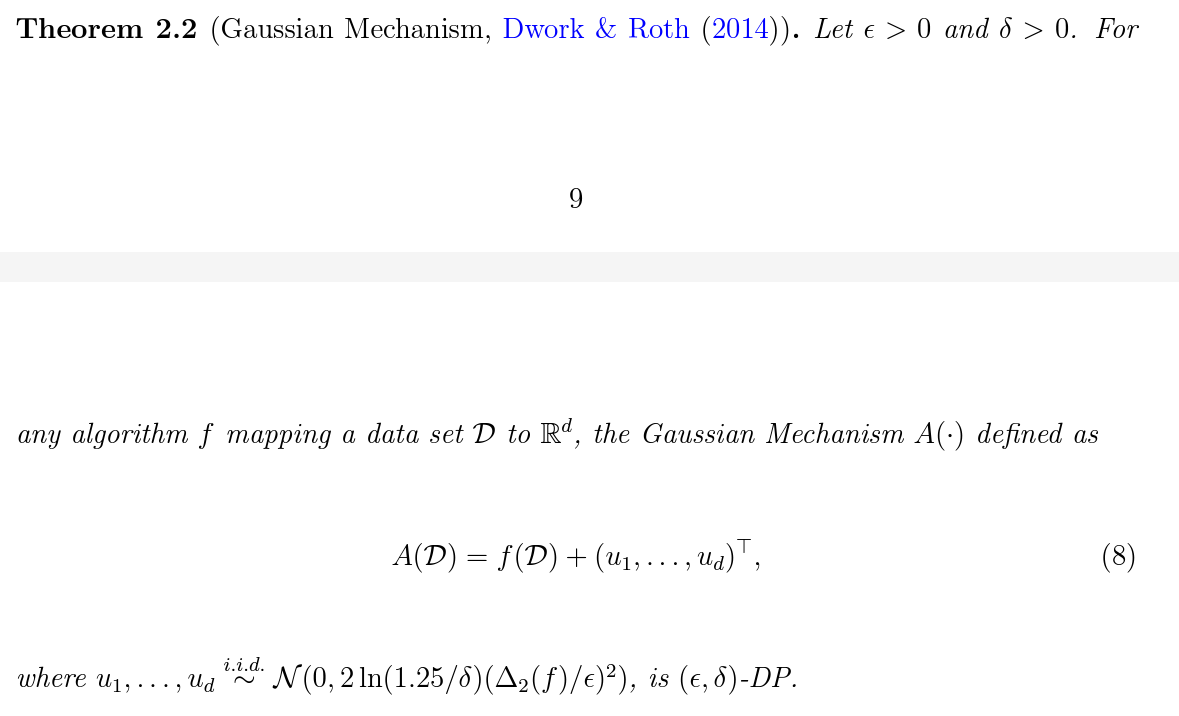
\includegraphics[width = 0.6\textwidth]{pic1.png}
    \caption{theorem}
    \label{fig:1}
\end{figure}
\newline
We can conclude that $M(x)-\overline{x}$ is $N(0,2\ln(1.25/\delta)(\Delta_2(f)/\epsilon)^2)$
\newline
$Pr[||M(x)-\overline{x}||_{\infty}\leq B]\geq 1-\beta$ is equal to $Pr[||M(x)-\overline{x}||_{\infty}>B]< \beta$.
This is equal to $Pr[\max\limits_{i\in [d]}|M(x)-\overline{x}|>B]<\beta$.
\newline
Use \textbf{union bound}, if we can get $d\cdot Pr[|M(x)-\overline{x}|>B]<\beta$, then we have $Pr[\max\limits_{i\in [d]}|M(x)-\overline{x}|>B]\leq d\cdot Pr[|M(x)-\overline{x}|>B]<\beta$
\newline
Use \textbf{Chernoff bound}:$P(X-\mu\geq a)\leq e^{-\frac{a^2}{2\sigma^2}}$, we can get $Pr[M(x)-\overline{x}>B]\leq e^{-\frac{B^2}{2\sigma^2}}$. So $Pr[|M(x)-\overline{x}|>B]\leq e^{-\frac{B^2}{\sigma^2}}$.
\newline
Let $\frac{\beta}{d}=e^{-\frac{B^2}{\sigma^2}}$.
Therefore, we can get $B=\sqrt{2\ln(1.25/\delta)\ln(d/\beta)}\frac{\Delta_2(f)}{\epsilon}$
\newline
In this question, $\Delta_2(f)=\frac{100\sqrt{d}}{n}$, so $B=\sqrt{2\ln(1.25/\delta)\ln(d/\beta)}\frac{100\sqrt{d}}{\epsilon n}$

\section{Q6}
\subsection{a}
According to the definition of $\{\epsilon_i\}_{i\in [n]}-PDP$:
$\frac{Pr[M_1(D)\in S_1]}{Pr[M_1(D')\in S_1]}\leq e^{\epsilon_i^{(1)}}$, $\frac{Pr[M_2(D)\in S_2]}{Pr[M_2(D')\in S_2]}\leq e^{\epsilon_i^{(2)}}$. Therefore,
$\frac{Pr[M_{1,2}(D)\in S_1\times S_2]}{Pr[M_{1,2}(D')\in S_1\times S_2]}=\frac{Pr[M_1(D)\in S_1]\times Pr[M_2(D)\in S_2]}{Pr[M_1(D')\in S_1]\times Pr[M_2(D')\in S_2]}\leq e^{\epsilon_i^{(1)}+ \epsilon_i^{(2)}}$.
\newline
Thus, publishing the result of both is $\{\epsilon_i^{(1)}+\epsilon_i^{(2)}\}_{i\in [n]}$-PDP
\subsection{b}
$\pi_i=\begin{cases}\frac{e^{\epsilon_i}-1}{e^t-1}& \text{$\epsilon_i$<t}\\ 1 & \text{otherwise} \end{cases}$
\newline
Let $D_{S_{-i}}$($D_{S_{+i}}$) denote the dataset resulting from removing(adding) the $i$-th element from $D_S$.
\newline
Let $DP$ denote any $t$-differentially private mechanism. 
\newline
Let $RS$ denote the procedure that samples each element. 
\newline
So the Sample mechanism can be defined as $M(D_S)=DP(RS(D_S))$
\newline
We want to prove $\frac{Pr[M(D_S)\in S]}{Pr[M(D_{S_{-i}})\in S]}\leq e^{\epsilon_i}$
\newline
$Pr[M(D_S)\in S]=\sum\limits_{Z\subset D_{S_{-i}}}(\pi_i\cdot Pr[RS(D_{S_{-i}})=Z]\cdot Pr[DP(D_{S_{+i}})\in S])+((1-\pi_i)\cdot Pr[M(D_{S_{-i}})\in S])$
\newline
Since $DP$ is $t$-differentially private, we can get $Pr[DP(D_{S_{+i}})\in S]\leq e^t\cdot Pr[DP(D_{S_i})\in S]$
\newline
Therefore, $Pr[M(D_S)\in S]\leq \sum\limits_{Z\subset D_{S_{-i}}}(\pi_i\cdot Pr[RS(D_{S_{-i}})=Z]\cdot e^t\cdot Pr[DP(D_{S_i})\in S])+((1-\pi_i)\cdot Pr[M(D_{S_{-i}})\in S])=\pi_i(e^t\cdot Pr[M(D_{S_{-i}})\in S])+(1-\pi_i)Pr[M(D_{S_{-i}})\in S]=(1-\pi_i+\pi_ie^t)Pr[M(D_{S_{-i}})\in S]$
\newline
\textbf{If $\epsilon_i\geq t$:}
\newline
We can get $\pi_i=1$, so $Pr[M(D_S)\in S]=(1-1+e^t)Pr[M(D_{S_{-i}})\in S]=e^tPr[M(D_{S_{-i}})\in S]\leq e^{\epsilon_i}Pr[M(D_{S_{-i}})\in S]$
\newline
\textbf{If $\epsilon_i<t$:}
\newline
We can get $\pi_i=\frac{e^{\epsilon_i}-1}{e^t-1}$, so $Pr[M(D_S)\in S]\leq \frac{e^{\epsilon_i}-1}{e^t-1}(e^tPr[M(D_{S_{-i}})\in S])+(1-\frac{e^{\epsilon_i}-1}{e^t-1})Pr[M(D_{S_{-i}})\in S]=e^{\epsilon_i}Pr[M(D_{S_{-i}})\in S]$
\newline
Thus, we prove that the Sample mechanism is $\{\epsilon_i\}_{i\in [n]}$-PDP.

\end{document}